\documentclass{standalone}
\usepackage{tikz}
\usetikzlibrary{patterns, positioning}

\begin{document}
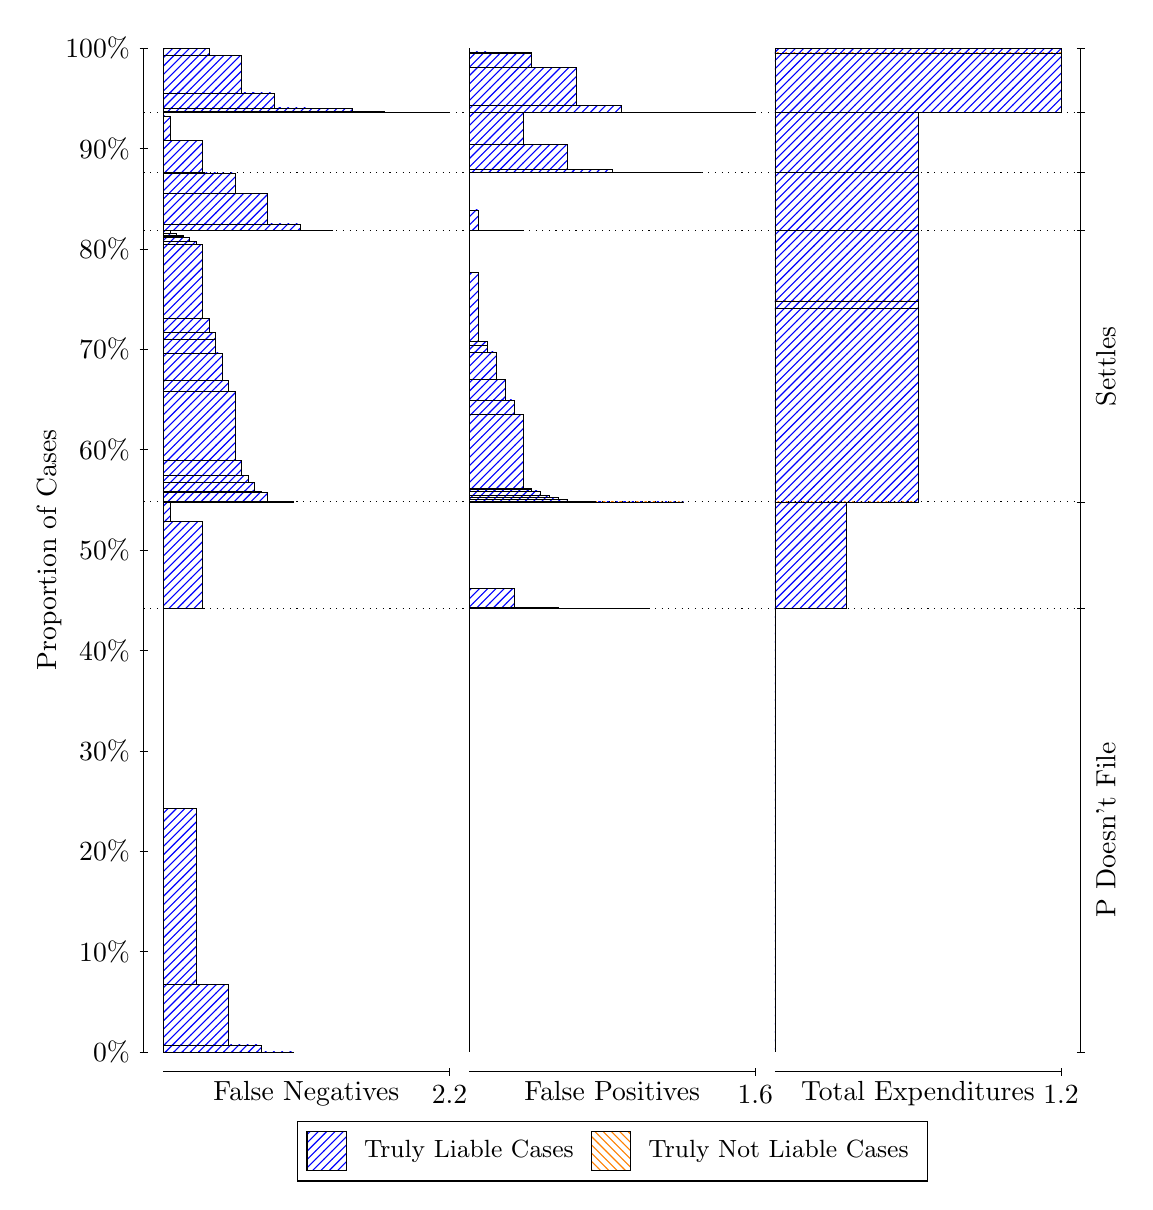
\begin{tikzpicture}
\draw[black, very thin] (1.5,1.75) -- (1.5,14.5);
\node[rotate=90, anchor=center] at (0.3, 8.125) {Proportion of Cases};
\draw[black, very thin] (1.45,1.75) -- (1.55,1.75);
\node[anchor=east] at (1.45, 1.75) {0\%};
\draw[black, very thin] (1.45,3.025) -- (1.55,3.025);
\node[anchor=east] at (1.45, 3.025) {10\%};
\draw[black, very thin] (1.45,4.3) -- (1.55,4.3);
\node[anchor=east] at (1.45, 4.3) {20\%};
\draw[black, very thin] (1.45,5.575) -- (1.55,5.575);
\node[anchor=east] at (1.45, 5.575) {30\%};
\draw[black, very thin] (1.45,6.85) -- (1.55,6.85);
\node[anchor=east] at (1.45, 6.85) {40\%};
\draw[black, very thin] (1.45,8.125) -- (1.55,8.125);
\node[anchor=east] at (1.45, 8.125) {50\%};
\draw[black, very thin] (1.45,9.4) -- (1.55,9.4);
\node[anchor=east] at (1.45, 9.4) {60\%};
\draw[black, very thin] (1.45,10.675) -- (1.55,10.675);
\node[anchor=east] at (1.45, 10.675) {70\%};
\draw[black, very thin] (1.45,11.95) -- (1.55,11.95);
\node[anchor=east] at (1.45, 11.95) {80\%};
\draw[black, very thin] (1.45,13.225) -- (1.55,13.225);
\node[anchor=east] at (1.45, 13.225) {90\%};
\draw[black, very thin] (1.45,14.5) -- (1.55,14.5);
\node[anchor=east] at (1.45, 14.5) {100\%};

\draw[black, very thin] (13.4,1.75) -- (13.4,14.5);
\draw[black, very thin] (13.35,1.75) -- (13.45,1.75);
\node[anchor=west] at (13.35, 1.75) {};
\draw[black, very thin] (13.35,7.3864) -- (13.45,7.3864);
\node[anchor=west] at (13.35, 7.3864) {};
\draw[black, very thin] (13.35,8.7374) -- (13.45,8.7374);
\node[anchor=west] at (13.35, 8.7374) {};
\draw[black, very thin] (13.35,12.18) -- (13.45,12.18);
\node[anchor=west] at (13.35, 12.18) {};
\draw[black, very thin] (13.35,12.917) -- (13.45,12.917);
\node[anchor=west] at (13.35, 12.917) {};
\draw[black, very thin] (13.35,13.683) -- (13.45,13.683);
\node[anchor=west] at (13.35, 13.683) {};
\draw[black, very thin] (13.35,14.5) -- (13.45,14.5);
\node[anchor=west] at (13.35, 14.5) {};

\draw[black, very thin, pattern color=blue, pattern=north east lines] (1.75,1.75) rectangle (3.4015,1.7509);
\draw[black, very thin, pattern color=blue, pattern=north east lines] (1.75,1.7509) rectangle (2.9886,1.8389);
\draw[black, very thin, pattern color=blue, pattern=north east lines] (1.75,1.8389) rectangle (2.5758,2.6101);
\draw[black, very thin, pattern color=blue, pattern=north east lines] (1.75,2.6101) rectangle (2.1629,4.8396);
\draw[black, very thin, pattern color=orange, pattern=north west lines] (1.75,4.8396) rectangle (1.75,4.8396);
\draw[black, very thin, pattern color=blue, pattern=north east lines] (1.75,4.8396) rectangle (1.75,7.3864);
\draw[black, very thin, pattern color=blue, pattern=north east lines] (1.75,7.3864) rectangle (2.2455,8.4888);
\draw[black, very thin, pattern color=blue, pattern=north east lines] (1.75,8.4888) rectangle (1.8326,8.7301);
\draw[black, very thin, pattern color=orange, pattern=north west lines] (1.75,8.7301) rectangle (1.75,8.7301);
\draw[black, very thin, pattern color=blue, pattern=north east lines] (1.75,8.7301) rectangle (1.75,8.7374);
\draw[black, very thin, pattern color=blue, pattern=north east lines] (1.75,8.7374) rectangle (3.4015,8.7404);
\draw[black, very thin, pattern color=blue, pattern=north east lines] (1.75,8.7404) rectangle (3.2364,8.7468);
\draw[black, very thin, pattern color=blue, pattern=north east lines] (1.75,8.7468) rectangle (3.0712,8.855);
\draw[black, very thin, pattern color=blue, pattern=north east lines] (1.75,8.855) rectangle (2.9886,8.8771);
\draw[black, very thin, pattern color=blue, pattern=north east lines] (1.75,8.8771) rectangle (2.9061,8.982);
\draw[black, very thin, pattern color=blue, pattern=north east lines] (1.75,8.982) rectangle (2.8235,9.0698);
\draw[black, very thin, pattern color=blue, pattern=north east lines] (1.75,9.0698) rectangle (2.7409,9.2707);
\draw[black, very thin, pattern color=blue, pattern=north east lines] (1.75,9.2707) rectangle (2.6583,10.142);
\draw[black, very thin, pattern color=blue, pattern=north east lines] (1.75,10.142) rectangle (2.5758,10.276);
\draw[black, very thin, pattern color=blue, pattern=north east lines] (1.75,10.276) rectangle (2.4932,10.629);
\draw[black, very thin, pattern color=blue, pattern=north east lines] (1.75,10.629) rectangle (2.4106,10.798);
\draw[black, very thin, pattern color=blue, pattern=north east lines] (1.75,10.798) rectangle (2.4106,10.886);
\draw[black, very thin, pattern color=blue, pattern=north east lines] (1.75,10.886) rectangle (2.328,11.071);
\draw[black, very thin, pattern color=blue, pattern=north east lines] (1.75,11.071) rectangle (2.2455,12.01);
\draw[black, very thin, pattern color=blue, pattern=north east lines] (1.75,12.01) rectangle (2.1629,12.04);
\draw[black, very thin, pattern color=blue, pattern=north east lines] (1.75,12.04) rectangle (2.0803,12.099);
\draw[black, very thin, pattern color=blue, pattern=north east lines] (1.75,12.099) rectangle (1.9977,12.106);
\draw[black, very thin, pattern color=blue, pattern=north east lines] (1.75,12.106) rectangle (1.9977,12.123);
\draw[black, very thin, pattern color=blue, pattern=north east lines] (1.75,12.123) rectangle (1.9152,12.146);
\draw[black, very thin, pattern color=blue, pattern=north east lines] (1.75,12.146) rectangle (1.8326,12.18);
\draw[black, very thin, pattern color=orange, pattern=north west lines] (1.75,12.18) rectangle (1.75,12.18);
\draw[black, very thin, pattern color=blue, pattern=north east lines] (1.75,12.18) rectangle (1.75,12.18);
\draw[black, very thin, pattern color=blue, pattern=north east lines] (1.75,12.18) rectangle (3.897,12.188);
\draw[black, very thin, pattern color=blue, pattern=north east lines] (1.75,12.188) rectangle (3.4841,12.266);
\draw[black, very thin, pattern color=blue, pattern=north east lines] (1.75,12.266) rectangle (3.0712,12.652);
\draw[black, very thin, pattern color=blue, pattern=north east lines] (1.75,12.652) rectangle (2.6583,12.914);
\draw[black, very thin, pattern color=blue, pattern=north east lines] (1.75,12.914) rectangle (2.2455,12.917);
\draw[black, very thin, pattern color=orange, pattern=north west lines] (1.75,12.917) rectangle (1.75,12.917);
\draw[black, very thin, pattern color=blue, pattern=north east lines] (1.75,12.917) rectangle (2.2455,13.323);
\draw[black, very thin, pattern color=blue, pattern=north east lines] (1.75,13.323) rectangle (1.8326,13.638);
\draw[black, very thin, pattern color=orange, pattern=north west lines] (1.75,13.638) rectangle (1.75,13.638);
\draw[black, very thin, pattern color=blue, pattern=north east lines] (1.75,13.638) rectangle (1.75,13.683);
\draw[black, very thin, pattern color=blue, pattern=north east lines] (1.75,13.683) rectangle (5.3833,13.683);
\draw[black, very thin, pattern color=blue, pattern=north east lines] (1.75,13.683) rectangle (4.9705,13.683);
\draw[black, very thin, pattern color=blue, pattern=north east lines] (1.75,13.683) rectangle (4.5576,13.697);
\draw[black, very thin, pattern color=blue, pattern=north east lines] (1.75,13.697) rectangle (4.1447,13.73);
\draw[black, very thin, pattern color=blue, pattern=north east lines] (1.75,13.73) rectangle (3.9795,13.73);
\draw[black, very thin, pattern color=blue, pattern=north east lines] (1.75,13.73) rectangle (3.7318,13.732);
\draw[black, very thin, pattern color=blue, pattern=north east lines] (1.75,13.732) rectangle (3.5667,13.74);
\draw[black, very thin, pattern color=blue, pattern=north east lines] (1.75,13.74) rectangle (3.3189,13.74);
\draw[black, very thin, pattern color=blue, pattern=north east lines] (1.75,13.74) rectangle (3.1538,13.93);
\draw[black, very thin, pattern color=blue, pattern=north east lines] (1.75,13.93) rectangle (2.9061,13.93);
\draw[black, very thin, pattern color=blue, pattern=north east lines] (1.75,13.93) rectangle (2.7409,14.41);
\draw[black, very thin, pattern color=blue, pattern=north east lines] (1.75,14.41) rectangle (2.328,14.498);
\draw[black, very thin, pattern color=blue, pattern=north east lines] (1.75,14.498) rectangle (1.9152,14.5);
\draw[black, very thin, pattern color=orange, pattern=north west lines] (1.75,14.5) rectangle (1.75,14.5);
\draw[black, very thin, pattern color=blue, pattern=north east lines] (1.75,14.5) rectangle (1.75,14.5);
\draw[black, very thin, pattern color=orange, pattern=north west lines] (5.6333,1.75) rectangle (5.6333,1.75);
\draw[black, very thin, pattern color=blue, pattern=north east lines] (5.6333,1.75) rectangle (5.6333,7.3864);
\draw[black, very thin, pattern color=orange, pattern=north west lines] (5.6333,7.3864) rectangle (7.9042,7.3864);
\draw[black, very thin, pattern color=blue, pattern=north east lines] (5.6333,7.3864) rectangle (7.9042,7.3864);
\draw[black, very thin, pattern color=blue, pattern=north east lines] (5.6333,7.3864) rectangle (7.3365,7.3864);
\draw[black, very thin, pattern color=blue, pattern=north east lines] (5.6333,7.3864) rectangle (6.7687,7.3937);
\draw[black, very thin, pattern color=blue, pattern=north east lines] (5.6333,7.3937) rectangle (6.201,7.635);
\draw[black, very thin, pattern color=blue, pattern=north east lines] (5.6333,7.635) rectangle (5.6333,8.7374);
\draw[black, very thin, pattern color=orange, pattern=north west lines] (5.6333,8.7374) rectangle (8.3583,8.7374);
\draw[black, very thin, pattern color=blue, pattern=north east lines] (5.6333,8.7374) rectangle (8.3583,8.7374);
\draw[black, very thin, pattern color=orange, pattern=north west lines] (5.6333,8.7374) rectangle (8.1313,8.7374);
\draw[black, very thin, pattern color=blue, pattern=north east lines] (5.6333,8.7374) rectangle (8.1313,8.7374);
\draw[black, very thin, pattern color=orange, pattern=north west lines] (5.6333,8.7374) rectangle (7.9042,8.7374);
\draw[black, very thin, pattern color=blue, pattern=north east lines] (5.6333,8.7374) rectangle (7.9042,8.7374);
\draw[black, very thin, pattern color=blue, pattern=north east lines] (5.6333,8.7374) rectangle (7.7906,8.7374);
\draw[black, very thin, pattern color=orange, pattern=north west lines] (5.6333,8.7374) rectangle (7.6771,8.7374);
\draw[black, very thin, pattern color=blue, pattern=north east lines] (5.6333,8.7374) rectangle (7.6771,8.7374);
\draw[black, very thin, pattern color=blue, pattern=north east lines] (5.6333,8.7374) rectangle (7.5635,8.7374);
\draw[black, very thin, pattern color=orange, pattern=north west lines] (5.6333,8.7374) rectangle (7.45,8.7374);
\draw[black, very thin, pattern color=blue, pattern=north east lines] (5.6333,8.7374) rectangle (7.45,8.7374);
\draw[black, very thin, pattern color=blue, pattern=north east lines] (5.6333,8.7374) rectangle (7.3365,8.7374);
\draw[black, very thin, pattern color=orange, pattern=north west lines] (5.6333,8.7374) rectangle (7.2229,8.7374);
\draw[black, very thin, pattern color=blue, pattern=north east lines] (5.6333,8.7374) rectangle (7.2229,8.7375);
\draw[black, very thin, pattern color=blue, pattern=north east lines] (5.6333,8.7375) rectangle (7.1094,8.7376);
\draw[black, very thin, pattern color=blue, pattern=north east lines] (5.6333,8.7376) rectangle (6.9958,8.7377);
\draw[black, very thin, pattern color=orange, pattern=north west lines] (5.6333,8.7377) rectangle (6.9958,8.7377);
\draw[black, very thin, pattern color=blue, pattern=north east lines] (5.6333,8.7377) rectangle (6.9958,8.7377);
\draw[black, very thin, pattern color=blue, pattern=north east lines] (5.6333,8.7377) rectangle (6.8823,8.7716);
\draw[black, very thin, pattern color=blue, pattern=north east lines] (5.6333,8.7716) rectangle (6.7687,8.7949);
\draw[black, very thin, pattern color=blue, pattern=north east lines] (5.6333,8.7949) rectangle (6.6552,8.8182);
\draw[black, very thin, pattern color=blue, pattern=north east lines] (5.6333,8.8182) rectangle (6.5417,8.8771);
\draw[black, very thin, pattern color=blue, pattern=north east lines] (5.6333,8.8771) rectangle (6.4281,8.8928);
\draw[black, very thin, pattern color=blue, pattern=north east lines] (5.6333,8.8928) rectangle (6.4281,8.9072);
\draw[black, very thin, pattern color=blue, pattern=north east lines] (5.6333,8.9072) rectangle (6.3146,9.8469);
\draw[black, very thin, pattern color=blue, pattern=north east lines] (5.6333,9.8469) rectangle (6.201,10.032);
\draw[black, very thin, pattern color=blue, pattern=north east lines] (5.6333,10.032) rectangle (6.0875,10.288);
\draw[black, very thin, pattern color=blue, pattern=north east lines] (5.6333,10.288) rectangle (5.974,10.642);
\draw[black, very thin, pattern color=blue, pattern=north east lines] (5.6333,10.642) rectangle (5.8604,10.721);
\draw[black, very thin, pattern color=blue, pattern=north east lines] (5.6333,10.721) rectangle (5.8604,10.776);
\draw[black, very thin, pattern color=blue, pattern=north east lines] (5.6333,10.776) rectangle (5.7469,11.647);
\draw[black, very thin, pattern color=blue, pattern=north east lines] (5.6333,11.647) rectangle (5.6333,12.18);
\draw[black, very thin, pattern color=orange, pattern=north west lines] (5.6333,12.18) rectangle (6.3146,12.18);
\draw[black, very thin, pattern color=blue, pattern=north east lines] (5.6333,12.18) rectangle (6.3146,12.183);
\draw[black, very thin, pattern color=blue, pattern=north east lines] (5.6333,12.183) rectangle (5.7469,12.445);
\draw[black, very thin, pattern color=blue, pattern=north east lines] (5.6333,12.445) rectangle (5.6333,12.917);
\draw[black, very thin, pattern color=orange, pattern=north west lines] (5.6333,12.917) rectangle (8.5854,12.917);
\draw[black, very thin, pattern color=blue, pattern=north east lines] (5.6333,12.917) rectangle (8.5854,12.917);
\draw[black, very thin, pattern color=blue, pattern=north east lines] (5.6333,12.917) rectangle (8.0177,12.918);
\draw[black, very thin, pattern color=blue, pattern=north east lines] (5.6333,12.918) rectangle (7.45,12.962);
\draw[black, very thin, pattern color=blue, pattern=north east lines] (5.6333,12.962) rectangle (6.8823,13.276);
\draw[black, very thin, pattern color=blue, pattern=north east lines] (5.6333,13.276) rectangle (6.3146,13.683);
\draw[black, very thin, pattern color=orange, pattern=north west lines] (5.6333,13.683) rectangle (9.2667,13.683);
\draw[black, very thin, pattern color=blue, pattern=north east lines] (5.6333,13.683) rectangle (9.2667,13.683);
\draw[black, very thin, pattern color=orange, pattern=north west lines] (5.6333,13.683) rectangle (8.699,13.683);
\draw[black, very thin, pattern color=blue, pattern=north east lines] (5.6333,13.683) rectangle (8.699,13.683);
\draw[black, very thin, pattern color=orange, pattern=north west lines] (5.6333,13.683) rectangle (8.1313,13.683);
\draw[black, very thin, pattern color=blue, pattern=north east lines] (5.6333,13.683) rectangle (8.1313,13.685);
\draw[black, very thin, pattern color=blue, pattern=north east lines] (5.6333,13.685) rectangle (7.5635,13.773);
\draw[black, very thin, pattern color=orange, pattern=north west lines] (5.6333,13.773) rectangle (7.5635,13.773);
\draw[black, very thin, pattern color=blue, pattern=north east lines] (5.6333,13.773) rectangle (7.5635,13.773);
\draw[black, very thin, pattern color=blue, pattern=north east lines] (5.6333,13.773) rectangle (6.9958,14.251);
\draw[black, very thin, pattern color=blue, pattern=north east lines] (5.6333,14.251) rectangle (6.9958,14.252);
\draw[black, very thin, pattern color=orange, pattern=north west lines] (5.6333,14.252) rectangle (6.7687,14.252);
\draw[black, very thin, pattern color=blue, pattern=north east lines] (5.6333,14.252) rectangle (6.7687,14.252);
\draw[black, very thin, pattern color=blue, pattern=north east lines] (5.6333,14.252) rectangle (6.4281,14.433);
\draw[black, very thin, pattern color=blue, pattern=north east lines] (5.6333,14.433) rectangle (6.4281,14.442);
\draw[black, very thin, pattern color=orange, pattern=north west lines] (5.6333,14.442) rectangle (6.201,14.442);
\draw[black, very thin, pattern color=blue, pattern=north east lines] (5.6333,14.442) rectangle (6.201,14.442);
\draw[black, very thin, pattern color=blue, pattern=north east lines] (5.6333,14.442) rectangle (5.8604,14.449);
\draw[black, very thin, pattern color=blue, pattern=north east lines] (5.6333,14.449) rectangle (5.8604,14.45);
\draw[black, very thin, pattern color=orange, pattern=north west lines] (5.6333,14.45) rectangle (5.6333,14.45);
\draw[black, very thin, pattern color=blue, pattern=north east lines] (5.6333,14.45) rectangle (5.6333,14.5);
\draw[black, very thin, pattern color=orange, pattern=north west lines] (9.5167,1.75) rectangle (9.5167,1.75);
\draw[black, very thin, pattern color=blue, pattern=north east lines] (9.5167,1.75) rectangle (9.5167,7.3864);
\draw[black, very thin, pattern color=orange, pattern=north west lines] (9.5167,7.3864) rectangle (10.425,7.3864);
\draw[black, very thin, pattern color=blue, pattern=north east lines] (9.5167,7.3864) rectangle (10.425,8.7374);
\draw[black, very thin, pattern color=orange, pattern=north west lines] (9.5167,8.7374) rectangle (11.333,8.7374);
\draw[black, very thin, pattern color=blue, pattern=north east lines] (9.5167,8.7374) rectangle (11.333,11.195);
\draw[black, very thin, pattern color=orange, pattern=north west lines] (9.5167,11.195) rectangle (11.333,11.195);
\draw[black, very thin, pattern color=blue, pattern=north east lines] (9.5167,11.195) rectangle (11.333,11.289);
\draw[black, very thin, pattern color=orange, pattern=north west lines] (9.5167,11.289) rectangle (11.333,11.289);
\draw[black, very thin, pattern color=blue, pattern=north east lines] (9.5167,11.289) rectangle (11.333,12.18);
\draw[black, very thin, pattern color=orange, pattern=north west lines] (9.5167,12.18) rectangle (11.333,12.18);
\draw[black, very thin, pattern color=blue, pattern=north east lines] (9.5167,12.18) rectangle (11.333,12.917);
\draw[black, very thin, pattern color=orange, pattern=north west lines] (9.5167,12.917) rectangle (11.333,12.917);
\draw[black, very thin, pattern color=blue, pattern=north east lines] (9.5167,12.917) rectangle (11.333,13.683);
\draw[black, very thin, pattern color=orange, pattern=north west lines] (9.5167,13.683) rectangle (13.15,13.683);
\draw[black, very thin, pattern color=blue, pattern=north east lines] (9.5167,13.683) rectangle (13.15,14.438);
\draw[black, very thin, pattern color=orange, pattern=north west lines] (9.5167,14.438) rectangle (13.15,14.438);
\draw[black, very thin, pattern color=blue, pattern=north east lines] (9.5167,14.438) rectangle (13.15,14.5);
\draw[black, dotted] (1.5,7.3864) -- (13.4,7.3864);
\draw[black, dotted] (1.5,8.7374) -- (13.4,8.7374);
\draw[black, dotted] (1.5,12.18) -- (13.4,12.18);
\draw[black, dotted] (1.5,12.917) -- (13.4,12.917);
\draw[black, dotted] (1.5,13.683) -- (13.4,13.683);
\draw[black, very thin] (1.75,1.5) -- (5.3833,1.5);
\node[anchor=north] at (3.5667, 1.5) {False Negatives};
\draw[black, very thin] (5.3833,1.45) -- (5.3833,1.55);
\node[anchor=north] at (5.3833, 1.45) {2.2};

\draw[black, very thin] (5.6333,1.5) -- (9.2667,1.5);
\node[anchor=north] at (7.45, 1.5) {False Positives};
\draw[black, very thin] (9.2667,1.45) -- (9.2667,1.55);
\node[anchor=north] at (9.2667, 1.45) {1.6};

\draw[black, very thin] (9.5167,1.5) -- (13.15,1.5);
\node[anchor=north] at (11.333, 1.5) {Total Expenditures};
\draw[black, very thin] (13.15,1.45) -- (13.15,1.55);
\node[anchor=north] at (13.15, 1.45) {1.2};

\node[black, centered, rotate=90] at (13.72, 4.5682) {P Doesn't File};

\node[black, centered, rotate=90] at (13.72, 10.459) {Settles};




\draw (7.449999999999999,1.5) node[draw=none] (baseCoordinate) {};
\begin{scope}[align=center]
        \matrix[scale=0.5, draw=black, below=0.5cm of baseCoordinate, nodes={draw}, column sep=0.1cm]{
            \node[rectangle, draw, minimum width=0.5cm, minimum height=0.5cm, pattern=north east lines, pattern color=blue] {}; &
            \node[draw=none, font=\small] (B) {Truly Liable Cases}; &
            \node[rectangle, draw, minimum width=0.5cm, minimum height=0.5cm, pattern=north west lines, pattern color=orange] {}; &
            \node[draw=none, font=\small] (B) {Truly Not Liable Cases}; \\
            };
\end{scope}

\end{tikzpicture}
\end{document}